\documentclass[a0paper,blockverticalspace=25pt]{tikzposter}

\usepackage[most]{tcolorbox}
\usepackage{tikz}
\usepackage{svg}
\usepackage{amssymb}
\usepackage{amsmath}
\usepackage{fourier}
\usepackage{pifont}
% \usepackage[french]{babel}

\DeclareMathOperator*{\argmin}{argmin}

%% Tikzposter is highly customizable: please see
%% https://bitbucket.org/surmann/tikzposter/downloads/styleguide.pdf
\usetheme{Default}
\usetitlestyle{Filled}
\useblockstyle{TornOut}
\usebackgroundstyle{Empty}
\usenotestyle{VerticalShading}

\tikzposterlatexaffectionproofoff

% \usetikzlibrary{scopes}

%% Define Color Style

\definecolor{color1}{RGB}{221, 229, 182}
\definecolor{color2}{RGB}{96, 108, 56}
\definecolor{color3}{RGB}{172, 199, 157}
% \definecolor{other}{RGB}{134, 151, 79}
% \definecolor{trianglesup}{RGB}{221, 229, 182}

\definecolorstyle{myColorStyle}{
	\colorlet{colorOne}{color1}
	}{
	% Background Colors
	\colorlet{backgroundcolor}{colorOne!50}
	\colorlet{framecolor}{colorOne!50}
	% Title Colors
	\colorlet{titlefgcolor}{black}
	\colorlet{titlebgcolor}{colorOne}
	% Block Colors
	\colorlet{blocktitlebgcolor}{colorOne!50}
	\colorlet{blocktitlefgcolor}{black}
	\colorlet{blockbodybgcolor}{colorOne!50}
	\colorlet{blockbodyfgcolor}{black}
	% Innerblock Colors
	\colorlet{innerblocktitlebgcolor}{white}
	\colorlet{innerblocktitlefgcolor}{black}
	\colorlet{innerblockbodybgcolor}{white}
	\colorlet{innerblockbodyfgcolor}{black}
	% Note colors
	\colorlet{notefgcolor}{black}
	\colorlet{notebgcolor}{white}
	\colorlet{notefrcolor}{black}
}

\usecolorstyle{myColorStyle}

\definecolorstyle{bibStyle}{
	}{
	% Block Colors
	\colorlet{blocktitlebgcolor}{white}
	\colorlet{blockbodybgcolor}{white}
	\colorlet{blockbodyfgcolor}{white}
}

%% Set Title config

\usetikzlibrary{positioning}
\makeatletter
\def\title#1{\gdef\@title{\scalebox{\TP@titletextscale}{%
	\begin{minipage}[t]{\linewidth}
		\centering
		#1
		\par
		\vspace{0.5em}
	\end{minipage}%
}}}
\makeatother

\title{\parbox{\linewidth}{\Huge Combining Finite Element methods and Neural Networks to \\ solve elliptic problem on complex 2D geometries}}
\author{\parbox{\linewidth}{\Large \textbf{Frédérique LECOURTIER}, Emmanuel FRANCK, Michel DUPREZ, Vanessa LLERAS}}
\institute{}

\newtcbtheorem{mytheo}{Theorem}{colback=color1!30, % Couleur de fond de la boîte
	colframe=color3!90, % Couleur du cadre de la boîte
	arc=2mm, % Rayon de l'arrondi des coins
	boxrule=2pt, % Épaisseur du cadre de la boîte
	breakable, enhanced jigsaw,
	width=\linewidth,
	% opacityback=0.1
	}{th}

% \usepackage[square]{natbib}
% \bibliographystyle{dinat}
% % to remove "REFERENCES" title
% \usepackage{etoolbox}
% \patchcmd{\thebibliography}{\section*{\refname}}{}{}{}

\usepackage[backend=biber,style=alphabetic]{biblatex}
% Ajouter la ressource bibliographique
\addbibresource{biblio.bib}

\usepackage{hyperref}
\hypersetup{
	colorlinks=true,
	citecolor=color2,
	linkcolor=color2,
}

\begin{document}
	\maketitle[titletoblockverticalspace=20pt]
	\node [below left=6cm and 2cm] at (topright) {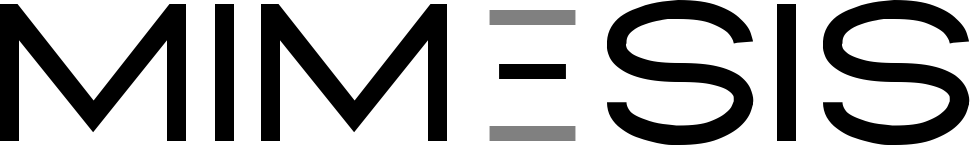
\includegraphics[width=15cm]{images/logo-mimesis.png}};

	\begin{frame}{Scientific context}
    \textbf{Context :} Create real-time digital twins of an organ (such as the liver).

    \textbf{$\phi$-FEM Method :} New fictitious domain finite element method.

    \begin{enumerate}[\ding{217}]
        \item domain given by a level-set function $\Rightarrow$ don't require a mesh fitting the boundary 
        \item allow to work on complex geometries 
        \item ensure geometric quality 
        % \item Cartesian grid adapted for neural networks
    \end{enumerate}
    
    \begin{center}
        \pgfimage[width=0.65\linewidth]{images/intro/context_geometry.png}
    \end{center}	

    \textit{Practical case:} Real-time simulation, shape optimization...
\end{frame}

\begin{frame}{Objective}
    \textbf{Current Objective :} Develop hybrid finite element / neural network methods.

	\begin{center}
		\begin{tcolorbox}[
			colback=white, % Couleur de fond de la boîte
			colframe=other, % Couleur du cadre de la boîte
			arc=2mm, % Rayon de l'arrondi des coins
			boxrule=0.5pt, % Épaisseur du cadre de la boîte
			breakable, enhanced jigsaw,
			width=0.8\linewidth
			]
			
			\textbf{OFFLINE :}
			
			\begin{figure}[htb]
				\centering
				\resizebox{\textwidth}{!}{%
					\begin{tikzpicture}
						\node at (0,0.8) {Several Geometries};
						\node[draw=none, inner sep=0pt] at (0,0) {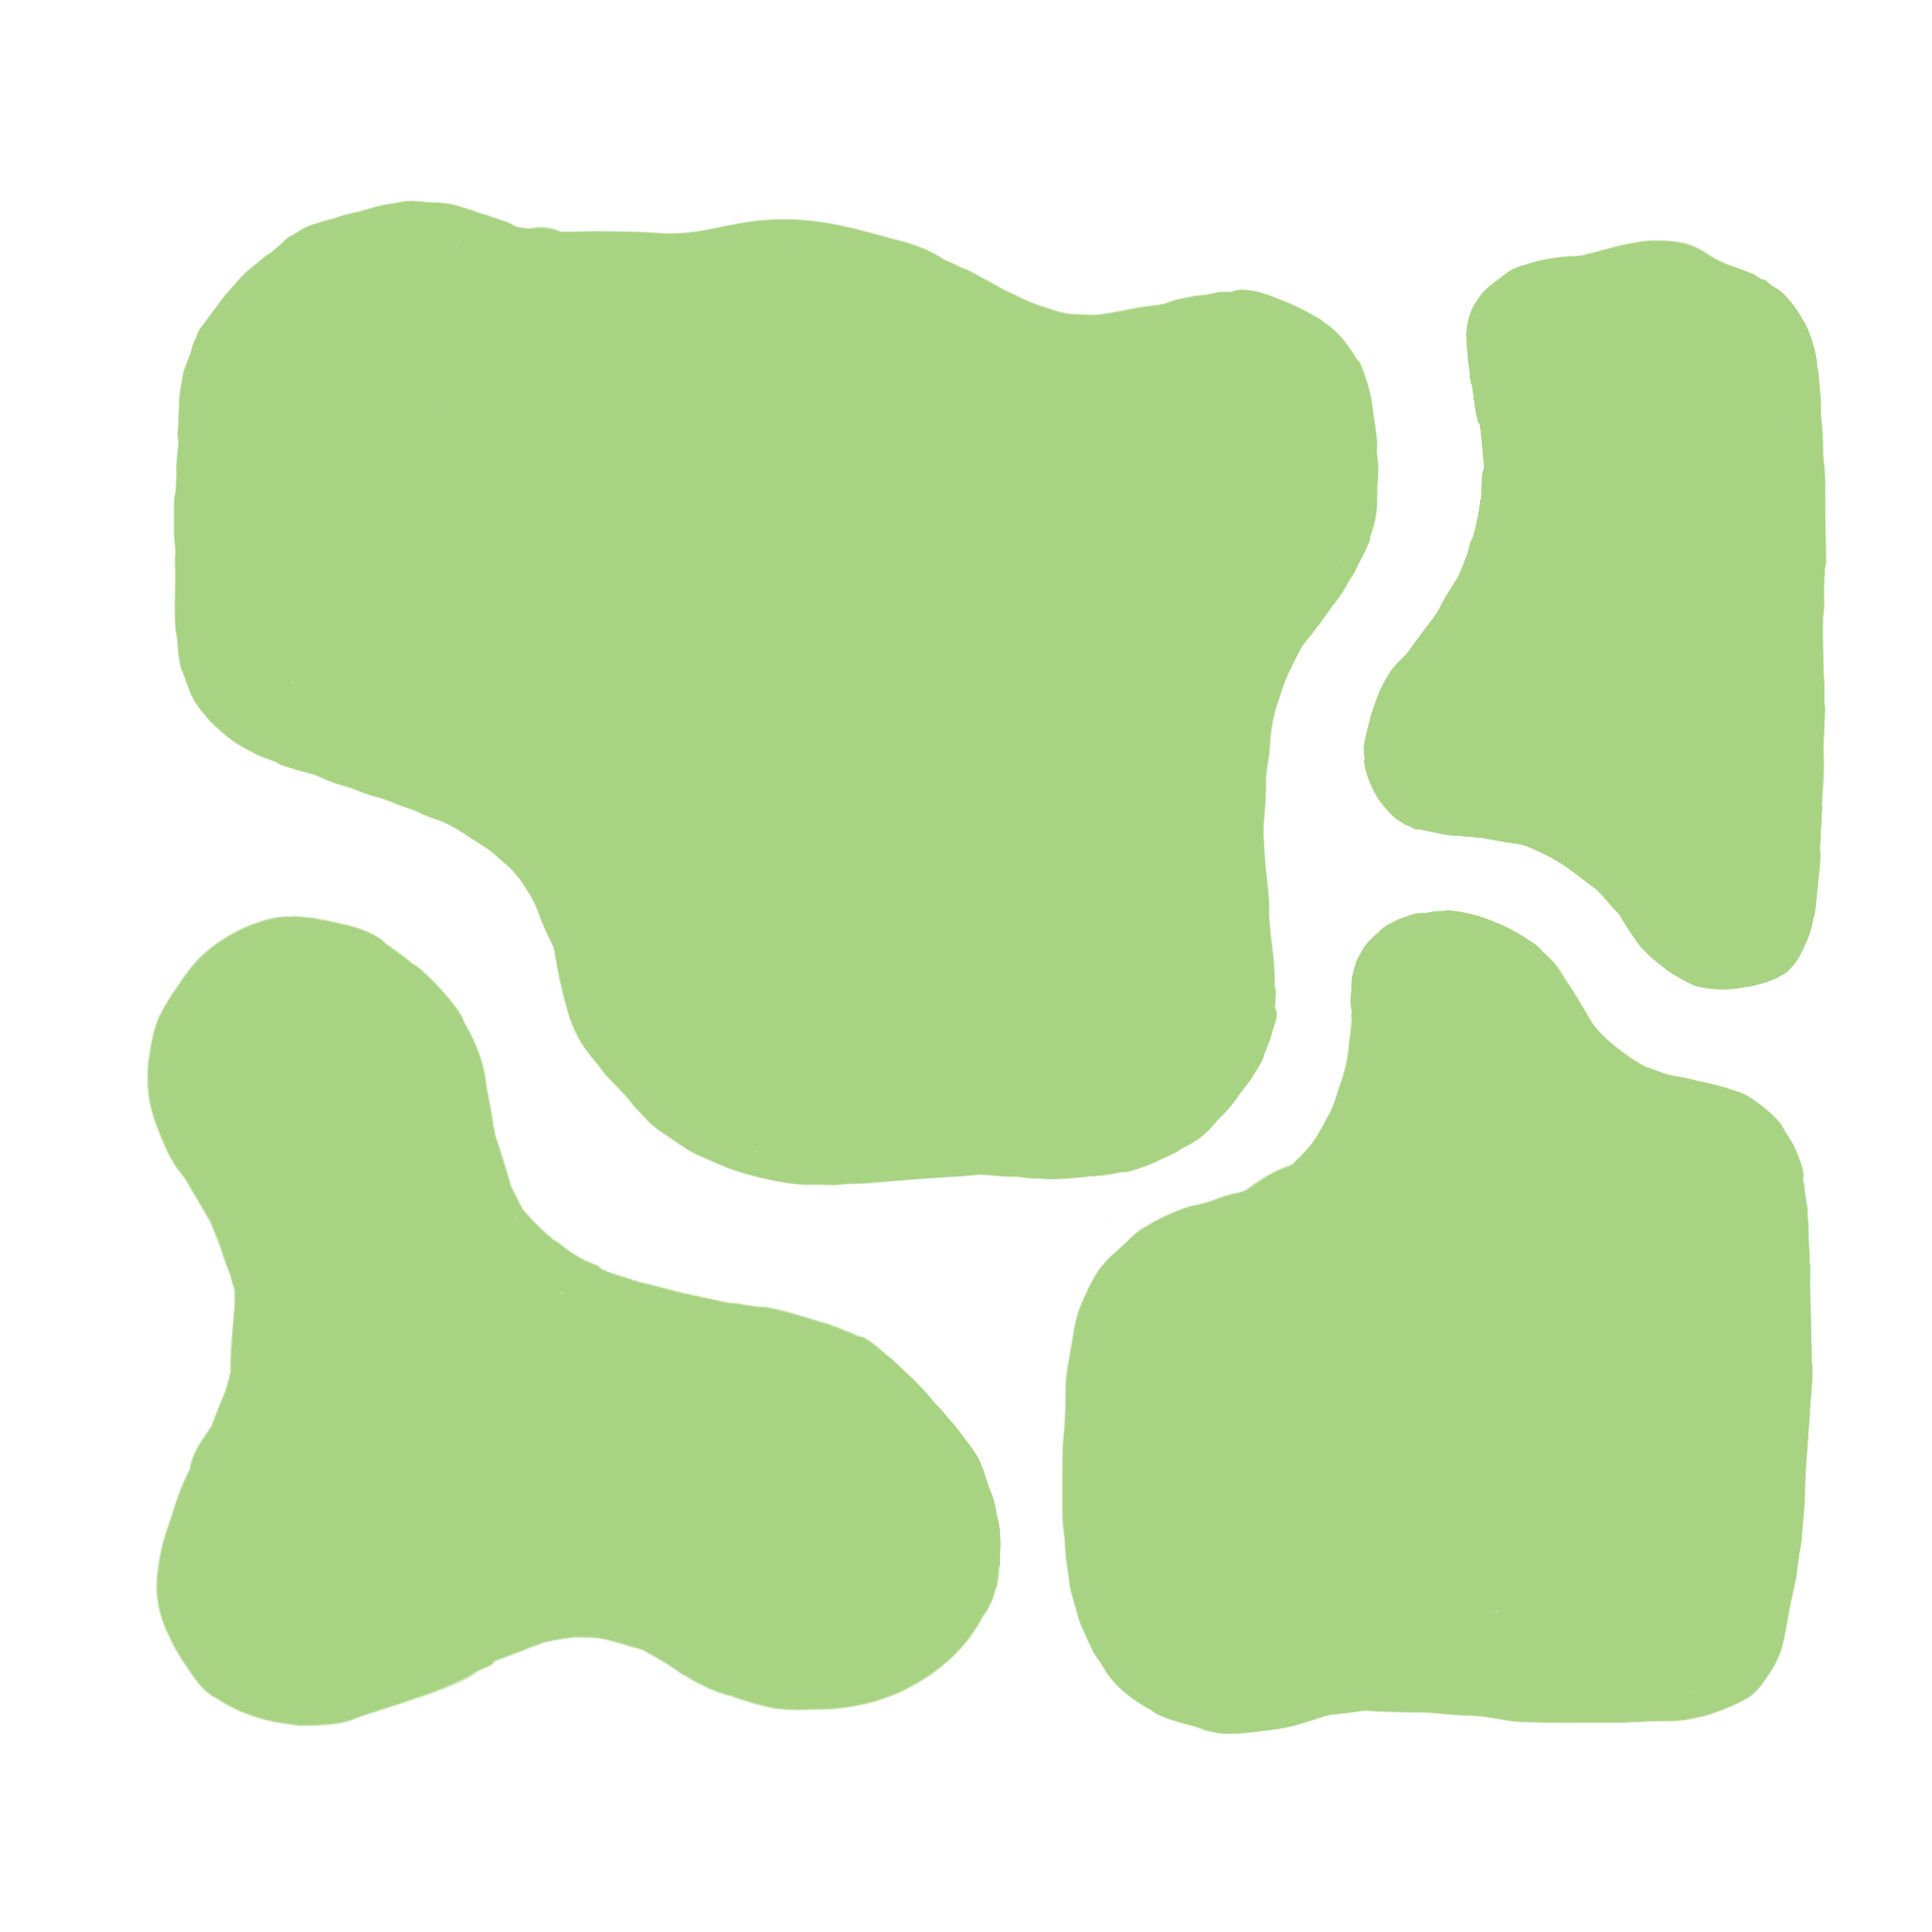
\includegraphics[width=2cm]{images/intro/objective_geom.png}};
						\node[title,font=\Large] at (1.6,0.1) {+};
						\node at (3.5,0.8) {Several Functions};
						\node[draw=none, inner sep=0pt] at (3.5,0) {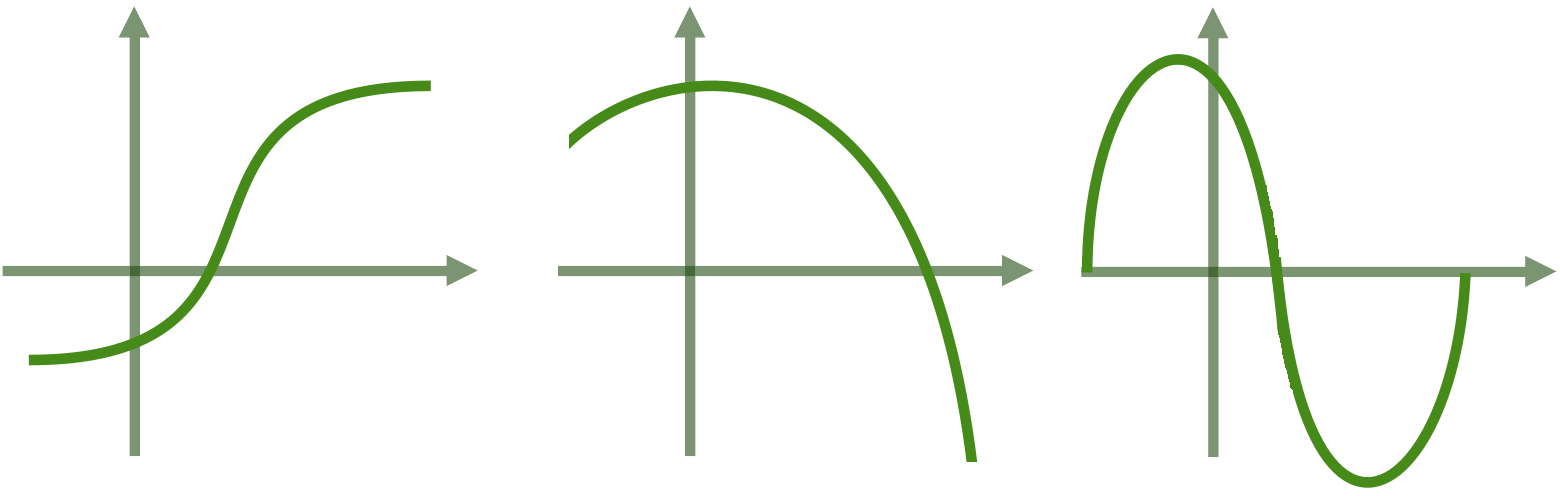
\includegraphics[width=3cm]{images/intro/objective_fct.png}};
						
						% Ajouter une flèche entre les deux rectangles
						\draw[->, title, line width=1.5pt] (5.5,0.1) -- (6.5,0.1);
						%		
						\node at (8,0.8) {Train a PINNs};
						\node[draw=none, inner sep=0pt] at (8,-0.1) {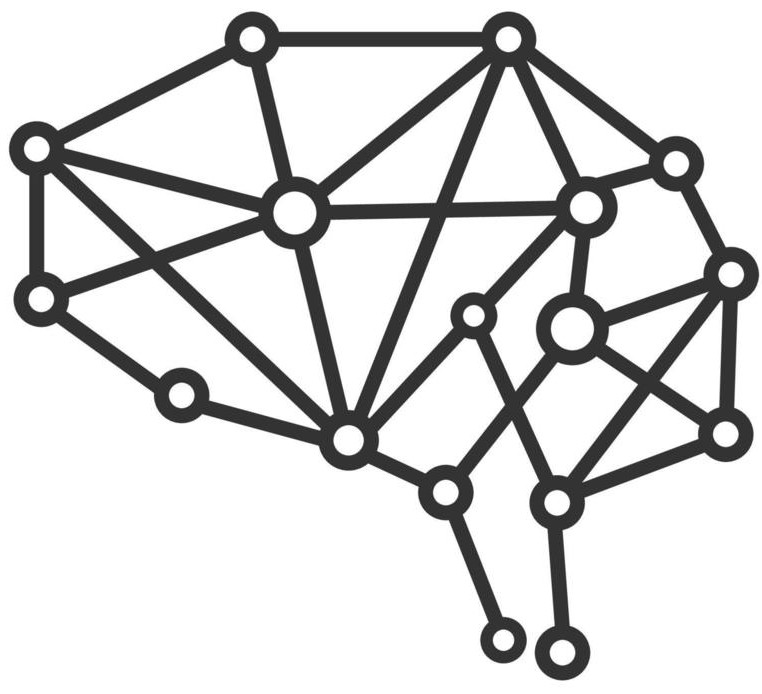
\includegraphics[width=1.5cm]{images/intro/objective_pinns.jpg}};				
					\end{tikzpicture}
				}%
			\end{figure}
			
			\textbf{ONLINE :}
			
			\vspace{-25pt}
			
			\begin{figure}[htb]
				\centering
				\resizebox{\textwidth}{!}{%
					\begin{tikzpicture}
						\node at (0,0.8) {1 Geometry - 1 Function};
						\node[draw=none, inner sep=0pt] at (0,0) {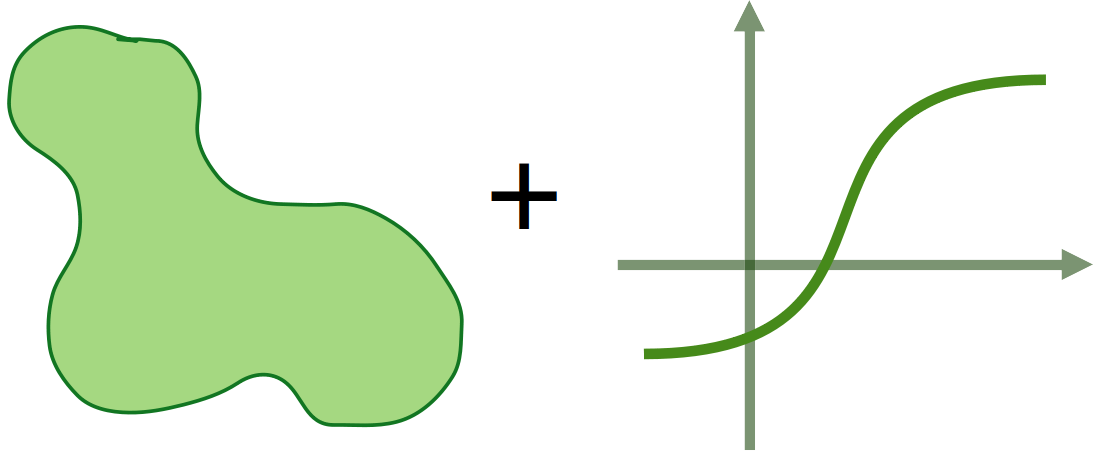
\includegraphics[width=2cm]{images/intro/objective_onegeom_onefct.png}};
						%		\node[title,font=\Large] at (1.6,0.1) {+};
						%		\node at (3.5,0.8) {Several Functions};
						%		\node[draw=none, inner sep=0pt] at (3.5,0) {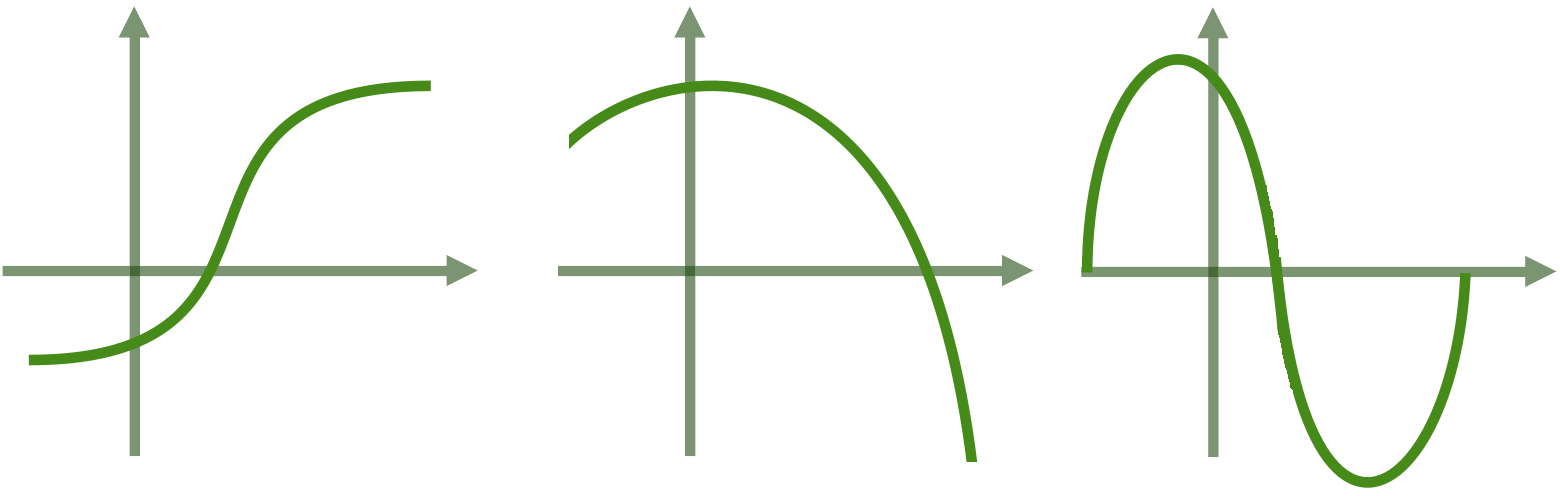
\includegraphics[width=3cm]{images/intro/objective_fct.png}};
						
						\draw[->, title, line width=1.5pt] (2,0.1) -- (3,0.1);
						
						\node[align=center] at (4,1) {Get PINNs \\ prediction};
						\node[draw=none, inner sep=0pt] at (4,-0.1) {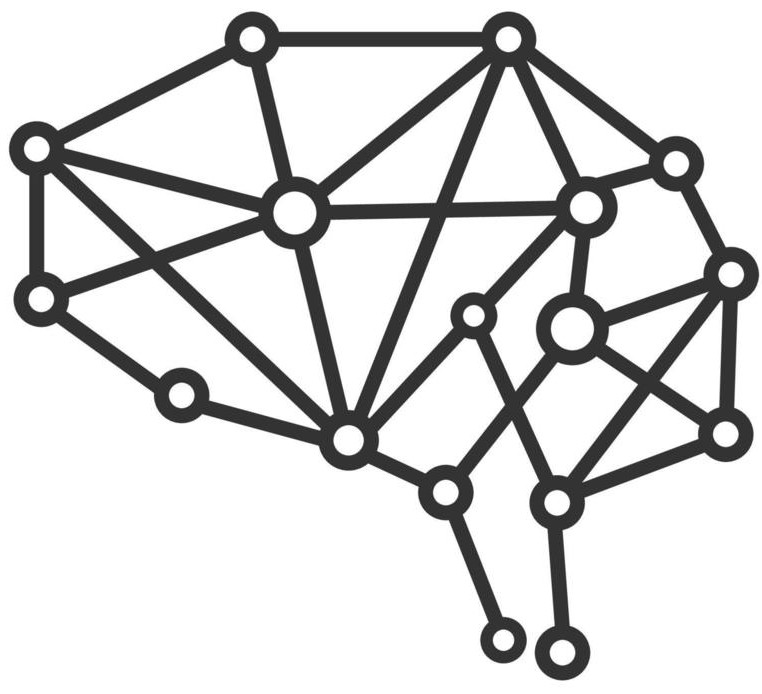
\includegraphics[width=1.5cm]{images/intro/objective_pinns.jpg}};
						
						% Ajouter une flèche entre les deux rectangles
						\draw[->, title, line width=1.5pt] (5.5,0.1) -- (6.5,0.1);
						%		
						\node[align=center] at (8,1) {Correct prediction \\ with $\phi$-FEM};
						\node[draw=none, inner sep=0pt] at (8,-0.1) {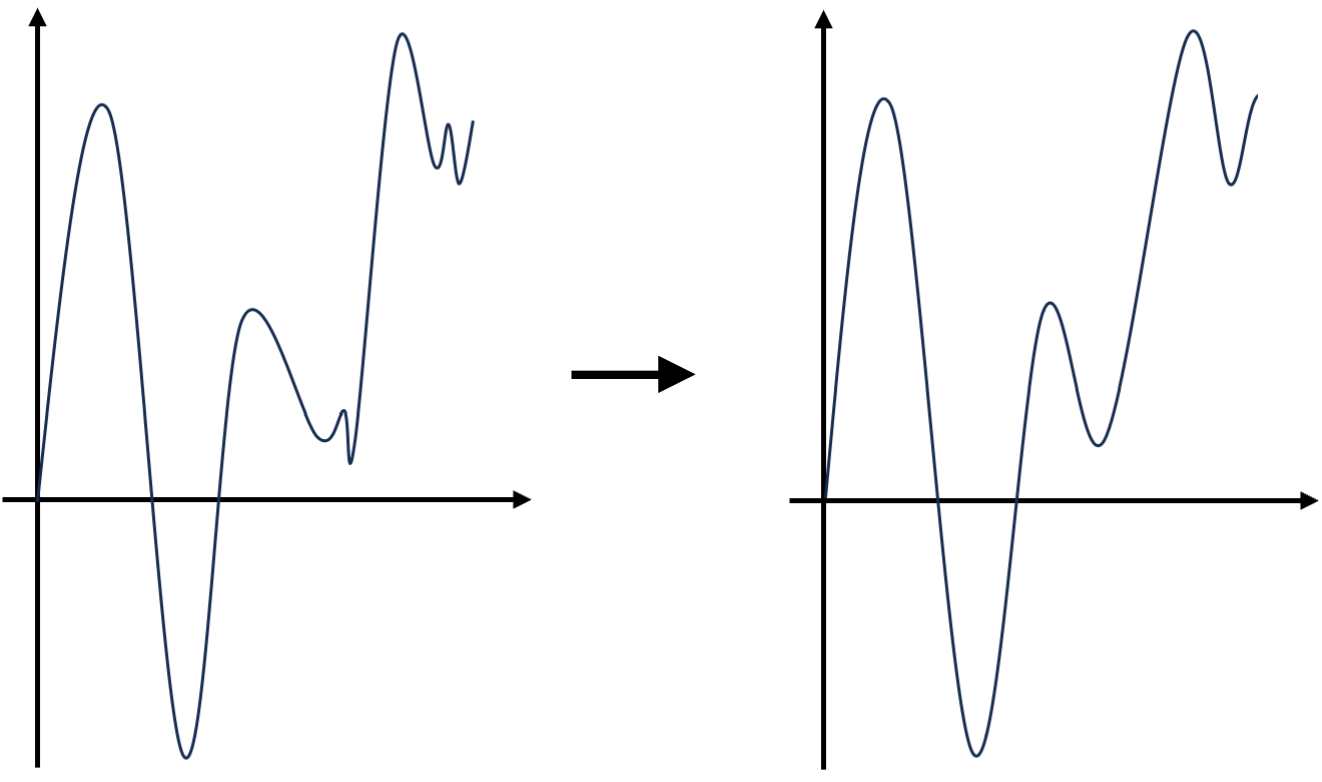
\includegraphics[width=2.5cm]{images/intro/objective_corr.png}};		
					\end{tikzpicture}
				}%
			\end{figure}
		\end{tcolorbox}
	\end{center}

    \textbf{Evolution :}

    \small
    % \setstretch{0.5}
    \begin{itemize}
        \item Geometry : 2D, simple, fixed (as circle, ellipse..) $ \; \rightarrow \;$ 3D / complex / variable
        \item PDE : simple, static (Poisson problem) $\; \rightarrow \;$ complex / dynamic (elasticity, hyper-elasticity)
        \item Neural Network : simple and defined everywhere (PINNs) $\; \rightarrow \;$ Neural Operator
    \end{itemize}
\end{frame}

\begin{frame}{Problem considered}
    \textbf{Elliptic problem with Dirichlet conditions :} \\
    Find $u : \Omega \rightarrow \mathbb{R}^d (d=1,2,3)$ such that
    \begin{equation}
    	\left\{\begin{aligned}
    		&L(u)=-\nabla \cdot (A(x) \nabla u(x)) + c(x)u(x) = f(x) \quad \text{in } \Omega, \\
    		&u(x) = g(x) \quad \text{on } \partial \Omega
    	\end{aligned}\right. \label{edp}
    \end{equation}
	with $A$ a definite positive coercivity condition and $c$ a scalar. We consider $\Delta$ the Laplace operator, $\Omega$ a smooth bounded open set and $\Gamma$ its boundary. 
    
    \textbf{Weak formulation :}
    \begin{equation*}
    	\text{Find } u\in V \text{ such that } a(u, v) = l (v) \forall v\in V
    \end{equation*}
    
    with
    \begin{align*}
    	a(u,v)&=\int_{\Omega} (A(x)\nabla u(x)) \cdot \nabla v(x) + c(x)u(x)v(x) \, dx \\
    	l(v)&=\int_{\Omega} f(x)v(x) \, dx
    \end{align*}
    
    \footnotesize
    \textit{Remark :} For simplicity, we will not consider 1st order terms. 

%    We will define by
%    \begin{equation*}
%        ||u_{ex}-u_{method}||_{0,\Omega}^{(rel)}=\frac{\int_\Omega (u_{ex}-u_{method})^2}{\int_\Omega u_{ex}^2}
%    \end{equation*}
%    the relative error between
%    \begin{itemize}
%        \item $u_{ex}$ : the exact solution  
%        \item $u_{method}$ : the solution obtained by a method \\
%        (can be : FEM or $\phi$-FEM, a correction solver or the prediction of an neural network).
%    \end{itemize}
\end{frame}

\begin{frame}{Numerical methods}
	\textbf{Objective :} Show that the philosophy behind most ofd the methods are the same.
	\begin{center}
		Mesh-based methods \hspace{5pt} // \hspace{5pt} Physically informed learning
	\end{center}
	
	\textbf{Numerical methods :} Discrete an infinite-dimensional problem (unknown = function) and solve it in a finite-dimensional space (unknown = vector).
	\begin{enumerate}[\textbullet]
		\item \textbf{Encoding :} we encode the problem in a finite-dimensional space
		\item \textbf{Approximation :} solve the problem in finite-dimensional space
		\item \textbf{Decoding :} bring the solution back into infinite dimensional space
	\end{enumerate}
	
	\begin{center}
		\begin{tabular}{|c|c|c|}
			\hline
			\textbf{Encoding} & \textbf{Approximation} & \textbf{Decoding} \\
			\hline
			$f \; \rightarrow \theta_f$ & $\theta_f \; \rightarrow \theta_u$ & $\theta_u \; \rightarrow u_\theta$ \\
			\hline
		\end{tabular}
	\end{center}
\end{frame}


	\block{How to deal with complex geometry in PINNs ?}{
    % \warning \textbf{In practice :} Not so easy ! We need to find \textbf{\fcolorbox{color1!50}{color1}{how to sample in the geometry}}.
    \begin{center}
        \begin{minipage}{0.49\linewidth}
            \centering
            \begin{tcolorbox}[
                colback=color1!50, % Couleur de fond de la boîte
                colframe=color2, % Couleur du cadre de la boîte
                arc=2mm, % Rayon de l'arrondi des coins
                boxrule=2pt, % Épaisseur du cadre de la boîte
                breakable, enhanced jigsaw,
                width=\linewidth
                ]            
                \textbf{Approach by levelset.} \cite{sukumar_exact_2022}
    
                \vspace{10pt}
    
                \begin{minipage}{0.38\linewidth}
                    \centering
                    \pgfimage[width=0.7\linewidth]{images/levelset/levelset.png}
                \end{minipage}
                \begin{minipage}{0.58\linewidth}
                    \textbf{\textit{Advantages :}} \\
                    \ding{217} Sample is easy in this case. \\
                    \ding{217} Allow to impose in hard the BC (no more $J_{\text{bc}}$) :
                    \vspace{-5pt}
                    \begin{equation*}
                        u_\theta(X)=\phi(X)w_\theta(X)+g(X)
                    \end{equation*}
                    with $\phi$ a levelset function and $w_\theta$ a NN.
                \end{minipage}
            \end{tcolorbox}
    
            \begin{tcolorbox}[
                colback=color1!50, % Couleur de fond de la boîte
                colframe=color2, % Couleur du cadre de la boîte
                arc=2mm, % Rayon de l'arrondi des coins
                boxrule=2pt, % Épaisseur du cadre de la boîte
                breakable, enhanced jigsaw,
                width=\linewidth
                ]            
                \textbf{Levelset considered.} A regularized Signed Distance Function (SDF).
    
                \begin{mytheo}{Eikonal equation.}{eik}
                    If we have a boundary domain $\Gamma$, the SDF is solution to:
                    
                    \begin{minipage}{0.7\linewidth}
                        \hspace{350pt}
                        $\left\{\begin{aligned}
                            &||\nabla\phi(X)||=1, \; X\in\mathcal{O} \\
                            &\phi(X)=0, \; X\in\Gamma \\
                            &\nabla\phi(X)=n, \; X\in\Gamma
                        \end{aligned}\right.$
                    \end{minipage}
                    \begin{minipage}{0.25\linewidth}
                        \centering
                        \pgfimage[width=0.7\linewidth]{images/levelset/points_normals.png}
                    \end{minipage}
                    
                    with $\mathcal{O}$ a box which contains $\Omega$ completely and $n$ the exterior normal to $\Gamma$.
                \end{mytheo}
                
                \textbf{How to do that ?} with a PINNs \cite{clemot_neural_2023}, by adding the following regularization term
                \vspace{-5pt}
                \begin{equation*}
                    J_{\text{reg}} = \int_\mathcal{O} |\Delta\phi|^2.
                \end{equation*} 
            \end{tcolorbox}
        \end{minipage}	
        \;
        \begin{minipage}{0.49\linewidth}
            \centering
            \begin{tcolorbox}[
                colback=color1!50, % Couleur de fond de la boîte
                colframe=color2, % Couleur du cadre de la boîte
                arc=2mm, % Rayon de l'arrondi des coins
                boxrule=2pt, % Épaisseur du cadre de la boîte
                breakable, enhanced jigsaw,
                width=\linewidth
                ]            
                \textbf{Result :} \textbf{\fcolorbox{color1!50}{color1}{Levelset learning.}}
                
                \vspace{2pt}
    
                \begin{minipage}{0.48\linewidth}
                    \centering
                    \pgfimage[width=0.8\linewidth]{images/levelset/cat_levelset_loss.png}
                \end{minipage} 
                \begin{minipage}{0.48\linewidth}
                    \centering
                    \pgfimage[width=0.8\linewidth]{images/levelset/cat_levelset.png}
                \end{minipage} 
            \end{tcolorbox}
    
            \begin{tcolorbox}[
                colback=color1!50, % Couleur de fond de la boîte
                colframe=color2, % Couleur du cadre de la boîte
                arc=2mm, % Rayon de l'arrondi des coins
                boxrule=2pt, % Épaisseur du cadre de la boîte
                breakable, enhanced jigsaw,
                width=\linewidth
                ]            
                \textbf{Result :} \textbf{\fcolorbox{color1!50}{color1}{Poisson on Cat.}}
    
                \ding{217} Solving (\ref{edp}) with $f=1$ (non parametric) and homogeneous Dirichlet BC ($g= 0$). \\
                \ding{217} Looking for $u_\theta = \phi w_\theta$ with $\phi$ the levelset learned.
    
                \vspace{2pt}
    
                \begin{minipage}{0.48\linewidth}
                    \centering
                    \pgfimage[width=0.8\linewidth]{images/levelset/cat_poisson_loss.png}
                \end{minipage} 
                \begin{minipage}{0.48\linewidth}
                    \centering
                    \pgfimage[width=0.9\linewidth]{images/levelset/cat_poisson.png}
                \end{minipage} 
            \end{tcolorbox}
        \end{minipage}
    \end{center}

}

% \node (manote){
\note[rotate=8, width = 11cm, targetoffsetx=26cm, targetoffsety=15.5cm, roundedcorners=30, linewidth=1pt]{No mesh, so easy to go on complex geometry !}
\node[below left=0cm and 12cm] at (topright) {
\includegraphics[width=2cm]{images/levelset/speaking.png}};
% };

% \begin{scope}[shift=(manote.south west), x={($0.1*(manote.south east)-0.1*(manote.south west)$)},
%      y={($0.1*(manote.north west)-0.1*(manote.south west)$)}]

%      \draw[lightgray, step=1](manote.south west) grid (manote.north east);

% \end{scope}

    


	\begin{columns}

    \column{0.5}

    \block{How can we improve PINNs prediction ? \\ \textnormal{\Large Using FEM-type methods}}{
        \vspace{-20pt}
        \begin{center}
            \begin{tcolorbox}[
                colback=color1!50, % Couleur de fond de la boîte
                colframe=color2, % Couleur du cadre de la boîte
                arc=2mm, % Rayon de l'arrondi des coins
                boxrule=2pt, % Épaisseur du cadre de la boîte
                breakable, enhanced jigsaw,
                width=\linewidth
                ]            
                \textbf{Additive approach.} Considering $u_{\theta}$ as the prediction of our PINNs for the Poisson problem, the correction problem consists in writing the solution as
                \begin{equation*}
                    \tilde{u}=u_{\theta}+\underset{\textcolor{orange}{\ll 1}}{\fcolorbox{orange}{color1!50}{$\tilde{C}$}}
                \end{equation*}

                \vspace{-20pt}

                and searching $\tilde{C}: \Omega \rightarrow \mathbb{R}^d$ such that
                \begin{equation}
                    \left\{\begin{aligned}
                        -\Delta \tilde{C}&=\tilde{f}, \; &&\text{in } \Omega, \\
                        \tilde{C}&=0, \; &&\text{on } \Gamma,
                    \end{aligned}\right. \label{corr_add} \tag{$\mathcal{P}^{+}$}
                \end{equation}

                \vspace{-10pt}

                with $\tilde{f}=f+\Delta u_{\theta}$.
            \end{tcolorbox}
    
            \begin{tcolorbox}[
                colback=color1!50, % Couleur de fond de la boîte
                colframe=color2, % Couleur du cadre de la boîte
                arc=2mm, % Rayon de l'arrondi des coins
                boxrule=2pt, % Épaisseur du cadre de la boîte
                breakable, enhanced jigsaw,
                width=\linewidth
                ]            
                \textbf{Poisson problem on Square.}
                
                \vspace{10pt}

                \ding{217} Considering homogeneous Dirichlet BC ($g=0$) and $\Omega=[-0.5\pi,0.5\pi]^2$. \\
                \ding{217} Analytical levelset function : $\quad \phi(x,y)=(x-0.5\pi)(x+0.5\pi)(y-0.5\pi)(y+0.5\pi)$ \\
                \ding{217} Analytical solution :               
                \vspace{-8pt}
                \begin{equation*}
                    u_{ex}(x,y)=\exp\left(-\frac{(x-\mu_1)^2+(y-\mu_2)^2}{2}\right)\sin(2x)\sin(2y)
                \end{equation*} 
                with $\mu_1,\mu_2\in[-0.5,0.5]$ (\textbf{\fcolorbox{color1!50}{color1}{parametric}}). 
            \end{tcolorbox}

            \begin{tcolorbox}[
                colback=color1!50, % Couleur de fond de la boîte
                colframe=color2, % Couleur du cadre de la boîte
                arc=2mm, % Rayon de l'arrondi des coins
                boxrule=2pt, % Épaisseur du cadre de la boîte
                breakable, enhanced jigsaw,
                width=\linewidth
                ]            
                \textbf{Theoretical results.} Considering $u_{\theta}$ as the prediction of our PINNs.

                \hypersetup{citecolor=white}

                \begin{center}
                    \begin{mytheo}{\cite{ours_2024}}{add}
                        We denote $u$ the solution of the Poisson problem and $u_h$ the discrete solution of the correction problem (\ref{corr_add}) with $V_h$ a $\mathbb{P}_k$ Lagrange space. Thus
                        \begin{equation*}
                            || u-u_h ||_0 \lesssim \fcolorbox{orange}{color1!30}{$\frac{|u-u_{\theta}|_{H^{k+1}}}{|u|_{H^{k+1}}}$} h^{k+1} |u|_{H^{k+1}}
                        \end{equation*}
                        \vspace{-5pt}
                        \hspace{485pt} \begin{minipage}{0.2\linewidth}
                            \large \textbf{\textcolor{orange}{$C_{\text{gain}}$}}
                        \end{minipage}
                    \end{mytheo}
                \end{center}

                \hypersetup{citecolor=color2}

                \textit{Remark :} The constant $C_{\text{gain}}$ shows that the closer the prior is to the solution, the lower the error constant associated with the method.
            \end{tcolorbox}
        \end{center}	
    }

    \usecolorstyle{bibStyle}
    \useblockstyle{Default}

	\block{
		\vspace{-40pt}
        \AtNextBibliography{\small}
		\printbibliography[heading=none]
	}

    \usecolorstyle{myColorStyle}
    \useblockstyle{TornOut}

    \column{0.5}

    \block{Results \textnormal{- Improve prediction}}{
        \vspace{-20pt}
        \begin{center}
            \begin{tcolorbox}[
                colback=color1!50, % Couleur de fond de la boîte
                colframe=color2, % Couleur du cadre de la boîte
                arc=2mm, % Rayon de l'arrondi des coins
                boxrule=2pt, % Épaisseur du cadre de la boîte
                breakable, enhanced jigsaw,
                width=\linewidth
                ]            
                \textbf{Theoretical results.} Taking $\mu_1=0.05$, $\mu_2=0.22$.

                \vspace{10pt}

                \begin{center}
                    \pgfimage[width=0.75\linewidth]{images/corr/cvg_case1.png}
                \end{center}
                
                \normalsize
                \textit{Remark :} We note N the number of nodes in each direction of the square.
            \end{tcolorbox}
    
            \begin{tcolorbox}[
                colback=color1!50, % Couleur de fond de la boîte
                colframe=color2, % Couleur du cadre de la boîte
                arc=2mm, % Rayon de l'arrondi des coins
                boxrule=2pt, % Épaisseur du cadre de la boîte
                breakable, enhanced jigsaw,
                width=\linewidth
                ]            
                \textbf{Gains on error using additive approach.}

                Considering a set of $n_p=50$ parameters : $\left\{\big(\mu_1^{(1)},\mu_2^{(1)}\big),\dots,\big(\mu_1^{(n_p)},\mu_2^{(n_p)}\big)\right\}$.
	
                \vspace{5pt}
                
                \hspace{20pt}\begin{minipage}{0.05\linewidth}
                    \normalsize
                    \flushright
                    \rotatebox[origin=b]{90}{\textbf{Solution $\mathbb{P}_1$}} 
                \end{minipage}
                \begin{minipage}{0.8\linewidth}
                    \centering
                    \pgfimage[width=0.9\linewidth]{images/corr/gains_P1.png}
                \end{minipage} 
            \end{tcolorbox}

            \begin{tcolorbox}[
                colback=color1!50, % Couleur de fond de la boîte
                colframe=color2, % Couleur du cadre de la boîte
                arc=2mm, % Rayon de l'arrondi des coins
                boxrule=2pt, % Épaisseur du cadre de la boîte
                breakable, enhanced jigsaw,
                width=\linewidth
                ]            
                \textbf{Time/error ratio.} Training time for PINNs : $t_{PINNs}\approx 240s$.

                \vspace{10pt}

                \ding{217} \textbf{At a given precision, how long does each method take to solve 1 problem ?}

                \begin{center}
                    \pgfimage[width=0.45\linewidth]{images/corr/time_error_tab.png}
                \end{center}

                \vspace{10pt}

                \ding{217} \textbf{How many parameters $n_p$ to make our method faster than FEM ?}

                \vspace{10pt}

                \begin{minipage}{0.48\linewidth}
                    Total time of Additive approach :
                    \vspace{-5pt}
                    $$Tot_{Add}=t_{PINNs}+n_p t_{Add}$$
                \end{minipage}
                \begin{minipage}{0.48\linewidth}
                    Total time of FEM :
                    \vspace{-5pt}
                    $$Tot_{FEM}=n_p t_{FEM}$$
                \end{minipage}

                \vspace{10pt}

                Let's suppose we want to achieve an \textbf{\fcolorbox{color1!50}{color1}{error of $1e-3$}}.
                
                \vspace{-10pt}

                \begin{equation*}
                    Tot_{Add}<Tot_{FEM} \quad \Rightarrow \quad n_p > \frac{t_{PINNs}}{t_{FEM}-t_{Add}}\approx 5.61\quad  \Rightarrow \quad \fcolorbox{orange}{color1!50}{$n_p=6$}
                \end{equation*}

                \vspace{10pt}
            \end{tcolorbox}
        \end{center}
    }

    % \usecolorstyle{bibStyle}
    % \useblockstyle{Default}

	% \block{
	% 	\vspace{-40pt}
	% 	\footnotesize
	% 	\printbibliography[heading=none]
	% }

\end{columns}

	\usecolorstyle{bibStyle}

	\block{
		\vspace{-40pt}
		\footnotesize
		\printbibliography[heading=none]
	}

\end{document}